% This is samplepaper.tex, a sample chapter demonstrating the
% LLNCS macro package for Springer Computer Science proceedings;
% Version 2.20 of 2017/10/04
%
\documentclass[runningheads]{llncs}
%
\usepackage{graphicx}
\usepackage{placeins}
\usepackage{float}
% Used for displaying a sample figure. If possible, figure files should
% be included in EPS format.
%
% If you use the hyperref package, please uncomment the following line
% to display URLs in blue roman font according to Springer's eBook style:
% \renewcommand\UrlFont{\color{blue}\rmfamily}

\begin{document}
%
\title{Immortals 2023 Extended Team Description Paper}
%
%\titlerunning{Abbreviated paper title}
% If the paper title is too long for the running head, you can set
% an abbreviated paper title here
%

\author{Ali Salehi \and
Mohammad Tabasi \and
Omid Najafi \and
Ali Amouzandeh \and
MohammadHossein Fazeli \and
MohammadAli Ghasemieh \and
MohammadReza Niknezhad \and
Mustafa Talaeezadeh}
%
\authorrunning{Immortals Robotics}
% First names are abbreviated in the running head.
% If there are more than two authors, 'et al.' is used.
%
\institute{
\url{http://www.immortals-robotics.com}
}
%
\maketitle              % typeset the header of the contribution
%
\begin{abstract}
%The abstract should briefly summarize the contents of the paper in
%15--250 words.
This paper describes the recent work done by the Immortals Robotics Team for the upcoming competitions including the RoboCup 2023.

\keywords{RoboCup 2023  \and Small Size League}
\end{abstract}
%
%
%
\section{Introduction}
The Immortals Small Size League team was founded in 2008 and participated for the first time in RoboCup 2009 in Graz. The team consists of computer and electrical engineers and currently focuses on the Small Size League.
 There have been some changes in the mechanics and electronics of the robots in the past years. The process can be seen in the previous years TDPs and ETDPs.~\cite{ref_ETDP2019}.
 
 This year, the team focused on modernizing the electronics and software architecture. Efforts were also made to resolve issues observed during recent competitions, including RoboCup 2018, Montréal. In addition to the current robot, there is a 3D-printed prototype robot that was presented in 2018 and has been improved and tested since then. The goal is to achieve a modular, flexible, and reliable platform that would reduce the maintenance and future development costs of the robots.


\begin{figure}
\centering
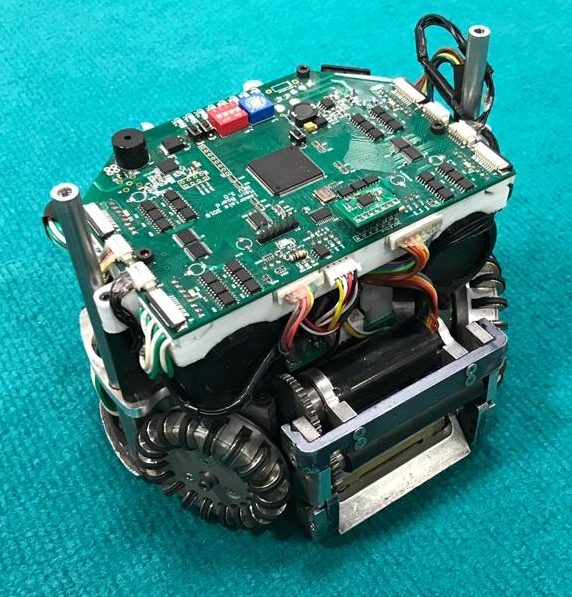
\includegraphics[width=10cm]{images/std_robot.jpeg}
\caption{Immortals current robot.} \label{fig_std_robot}
\end{figure}

Our team, Immortals, is thrilled to participate in this year's RoboCup SSL competition. With a history of innovation and success, we are constantly working to develop cutting-edge solutions in small-scale autonomous robotics. Building on our experience from last year's competition, we are currently dedicated to improving our AI software and robot electronics to address the needs we identified in our previous system. Our team is working tirelessly on designing and constructing a robot that will be smarter and more robust than ever before. Through an iterative process of development and testing, we are confident that we will create a robot team that is faster, smarter, and more agile than ever before. We look forward to showcasing our progress and competing against the best SSL teams from around the world.


\section{Kicking System}
Before 2018 the limit for the ball velocity was 8m/s. In order for robots to kick a ball that much fast, a strong shooting system including capacitors and solenoids where required. Since RoboCup 2018, Montréal, Canada, the maximum speed limit has been decreased to 6.5m/s which makes teams to wonder if they want to redesign their robots kicking system and optimize the space consumption or battery power in their robot. This year the Immortals robots kicking system has been modified in order to optimize the energy consumption from the battery. This way robots have the chance to stay longer in a match without the need of their batteries to get changed.


%%%%%%%%%%%%

\section{Electronics}

In 2018, changes were made to the electronics to modernize the designs and replace the old parts with their new counterparts. We tested them during RoboCup 2018, and the results show a solid improvement in reliability while reducing production costs. Currently, all robots use these circuits. The reader is referred to this team's previous year's TDP [1] for more details on the main circuit.\\
\indent This year, we're planning to redesign all of our electronics from scratch to reflect the latest developments in the league and also in the industry. The main goals are (1) reliability, (2) expandability, and (3) being more competitive. It should be mentioned that at the time of this writing, the design work is still ongoing and we don't have the final boards manufactured. We hope to equip at least half of our robots with the new parts in RoboCup 2023. We will publish the designs on our GitHub page shortly after the competition.

\begin{figure}
	\centering
	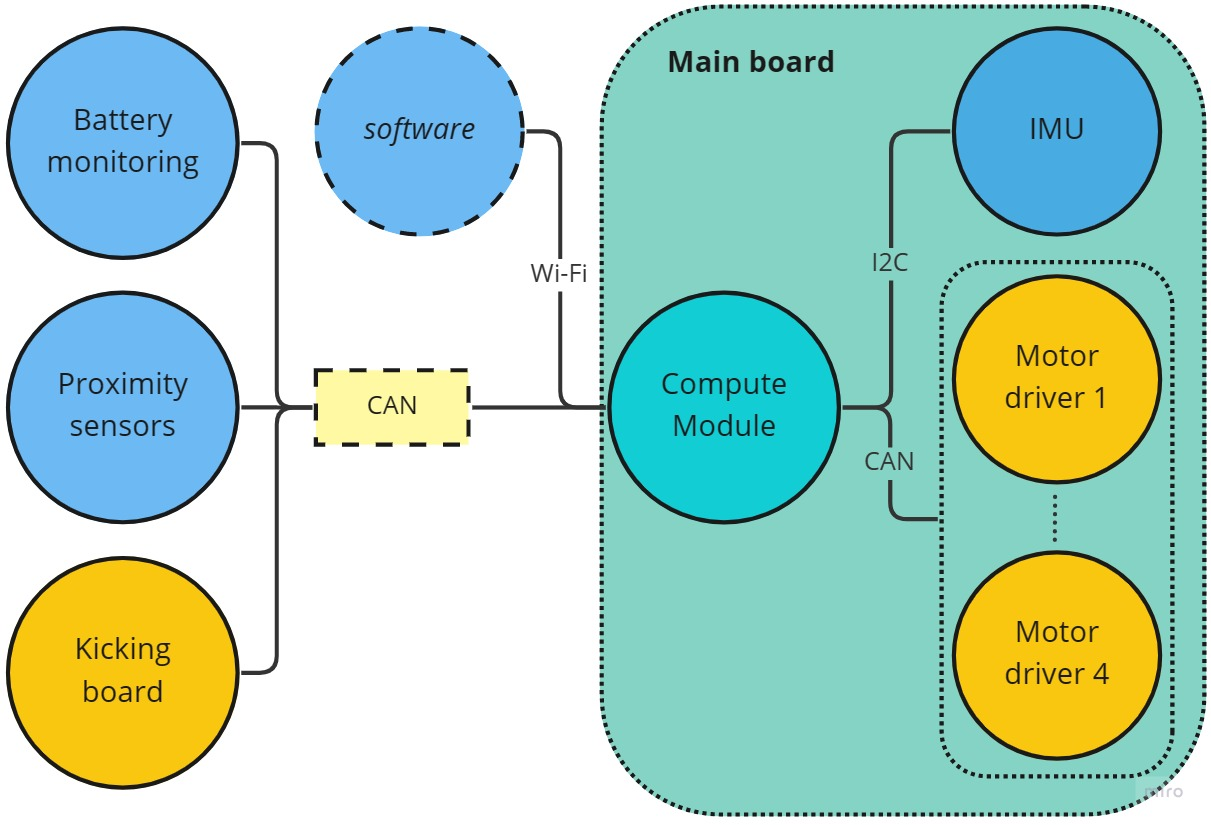
\includegraphics[width=0.8\textwidth]{images/electronics-architecture.jpg}
	\caption{The new electronics architecture}
	\label{fig:electronics-architecture}
\end{figure}

\subsection{Main board}
The current main board used by the team was designed in 2010 and has been used in its original form ever since, except for minor changes. It uses a Xilinx Spartan3 FPGA as the main and only processor. A soft processor (TSK3000) is used inside the FPGA to handle more sequential logic, while the FPGA itself is used to read encoders, drive BLDC motors, drive the boost converter, etc.
While this design is flexible and comparatively cheap to produce, it has shown its age in recent years. The main drawbacks are:
\begin{enumerate}
    \item The TSK3000 runs at around 36 MHz and in its current configuration is way too limited to develop any more sophisticated local processing and motion planning. Some efforts were done in the past to move parts of performance-critical C code to the logic gates, but it would make the implementation harder to change and extend. On the other hand the debugging workflow was too limiting, and any changes to the code needed a full rebuild of the FPGA project. All these factors resulted in the team using pretty much the same framework for several years, without being able to make major changes.
    \item The BLDC motor commutation is a simple 6-step trapezoidal commutation. It is easy to implement, but is inefficient and causes a high amount of torque ripple. Implementing a more sophisticated method, e.g. Field Oriented Control, requires massive changes to the PCB.
    \item We use nRF24L01 chip for wireless communication, with a custom payload layout on top of its Enhanced ShockBurst (ESB) protocol. This gives us a lot of flexibility, but being a low-level protocol means we need to add any higher-level feature needed, e.g. discovery.
    \item The waveform needed to drive the boost converter in the kicking board is generated by the FPGA. This meant that we were able to freely change it to match our needs, but in practice deemed too fragile.
    \item There are no current protections in the board. Any malfunction in the board itself or in another part of the robot, e.g. a stuck wheel, causes damage to the parts. This hugely reduces reliability and increases maintenance costs, and caused damage to the battery.
\end{enumerate}

To resolve these issues the work started on designing a new main board from scratch. The main features are:
\begin{enumerate}
    \item Raspberry Pi Compute Module 4 as the local compute unit on robot. We intend to move parts of the skill execution, data fusion and prediction, and motion planning to it.
    \item Raspberry Pi Compute Module's 5GHz WiFi as the wireless. This will greatly enhance the bandwidth and the feature-set of the link and will allow us to add robots as regular links to our software stack. This way they will receive world state and the AI output necessary to execute local skills.\\
    The latency characteristics of using WiFi instead of a low-level protocol in the lab environment has been satisfacroty. Using the default PCB-antenna at a distance of 20m to the access point, we were able to achieve a latency of ~2ms with a data loss of ~\%3. The latency requirements after moving more processing to the robot's local processor will be more relaxed. But, we are still considering adding a separate nRF chip to handle latency-sensitive if the new approach causes issues.
    \item CAN protocol will be used to connect the main board to other boards, including the kicking board, motor drivers, and the battery monioring board. This will give us a more robust and flexible base that we can build on top.
    \item 
\end{enumerate}

\subsection{Motor driver}
In the past competitions, motor driving ciruitury was one of the common failure points of the robot. As they were placed on the same PCB, the repair would require a complete reflow of the broken parts. In more severe cases, e.g. when the traces especially on the internal layers get damaged, it could mean the board will become irreparable.\\
This year we decided to design separate modular motor driving boards that will be placed on the main board for each motor. This will greatly enhance our ability to repair robots in case of a failure in one of the drivers. It would also make it easier to upgrade the main board and motor drivers separately.\\
This new driving board is based on:
\begin{enumerate}
    \item A dedicated BLDC driving IC, TMC4671. It implements  Field Oriented Control (FOC) for BLDC motors, and includes various closed-loop control methods. This offloads the local motor control functionality from the main MCU to the dedicated HW, which is more reliable in terms of latency. It has an SPI interface to receive both configuration and command, and send back sensory data including speed and position.
    \item A power mosfet driver IC, TMC6100. It drives the mosfets and senses the motor currents that is needed for the FOC algorithm. It also contains a fault detection mechanism.
    \item A small Arm processor, STM32F042G6Ux, that acts as a CAN client link to the main processor. It communicates with both the TMC4671 and the TMC6200 via SPI, and also reads the current sensor.
\end{enumerate}
\subsection{Kicking board}
In the previous years, we used a boost converter that was drived by the FPGA from the main board. There were also two discharge and a charged state pin connected directly to FPGA's IO pins. The were major issues with this design both in terms of reliability and charging performance.\\
This year we redesigned the kicking board with the following features:
\begin{enumerate}
    \item A dedicated flyback capacitor charging IC, LT3570, is used. This simplifies the design and improves performance and reliability at the same time. We use DA2034 transformer and the BSC109N10NS3G MOSFET.
    \item A STM32F042G6Ux MCU is used on the board to handle CAN protocol to the main board, and controls the charging IC, variable resistors, and discharge IGBTs.
    \item A high-power resistor network composed of three 2.4K 3W resistors is added to the board to discharge the capacitors when needed, without using the kicker magnets. The STN3N40K3 MOSFET drived by a ZXGD3009E6 is used to control the discharge.
    \item Two IGB50N60T IGBTs drived by a single IX4427MTR are used to discharge the capacitors to the kicking magnets. 
\end{enumerate}

\begin{figure}
	\centering
	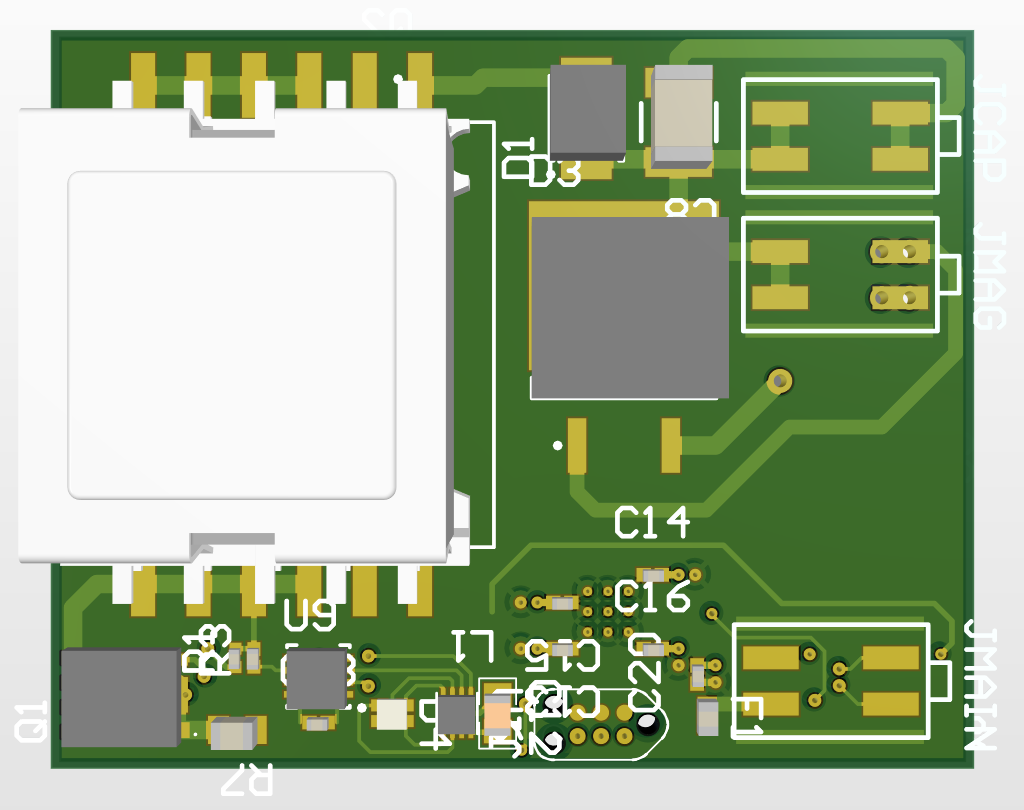
\includegraphics[width=0.6\textwidth]{images/mikona.png}
	\caption{The new kicking board design}
	\label{fig:MIKONA}
\end{figure}


\section{Software}
Our current software stack was developed in 2009 in C++ and has seen several additions and improvements throughout the years. This has resulted in a performant and robust software, and at the same time hard to maintain codebase that is too fragile to the new changes.\\
\indent This year the main focuses are to make our software:
\begin{enumerate}
    \item more robust
    \item easier to read/understand, and change/extend
    \item faster to iterate and extend
    \item more competitive
\end{enumerate}
In the following sections, we will describe the efforts made to reach these goals.

\subsection{Improving robustness}

\subsubsection{Third-party libraries}

This year we started using several third-party libraries for parts of our software:
\begin{enumerate}
    \item \textbf{\textit{Asio}}~\cite{ref_3rd-party_asio} for networking 
    \item \textbf{\textit{Quill}}~\cite{ref_3rd-party_quill} for logging
    \item \textbf{\textit{toml++}}~\cite{ref_3rd-party_tomlplusplus} for configuration files
    \item \textbf{\textit{Eigen}}~\cite{ref_3rd-party_eigen} for linear algebra
    \item \textbf{\textit{homog2d}}~\cite{ref_3rd-party_homog2d} for 2D math
\end{enumerate}

\indent Using these libraries over our custom solutions can help improve code quality, both in terms of robustness and ease of use.

\indent These open-source projects have a proven track record and have been extensively reviewed and stabilized by experts over time. This means they are more reliable than custom-built solutions and better suited to handle common tasks with reasonable performance and reliability.

\indent They also often come with a broader set of features that have detailed documentation, making them easier to integrate and use. This allows developers to focus on implementing the core logic without worrying about the underlying infrastructure. This results in more readable code that is less prone to bugs.

\subsection{Architecture}

Our current software is a single application that handles world state estimation, AI, and motion planning of the robots. This has the added benefit of being able to change the data flow between various parts quite easily. But forces us to implement everything in C++ to produce one single application that runs on one machine. Another side effect of such a monolithic design was that it encouraged more coupling between the soccer and the vision parts of the software and as a result made it harder to make changes to each of them.\\
\indent The goal this year is to refactor the codebase into separate parts that are connected via the network. This allows us to move the lower-level motion planning and skill execution to the robots' local processor, and develop GUIs using other technologies. \\
\indent At the time of writing this paper, this effort is still ongoing, but we are confident that we can make the transition to the new stack in time for RoboCup 2023.

\begin{figure}
	\centering
	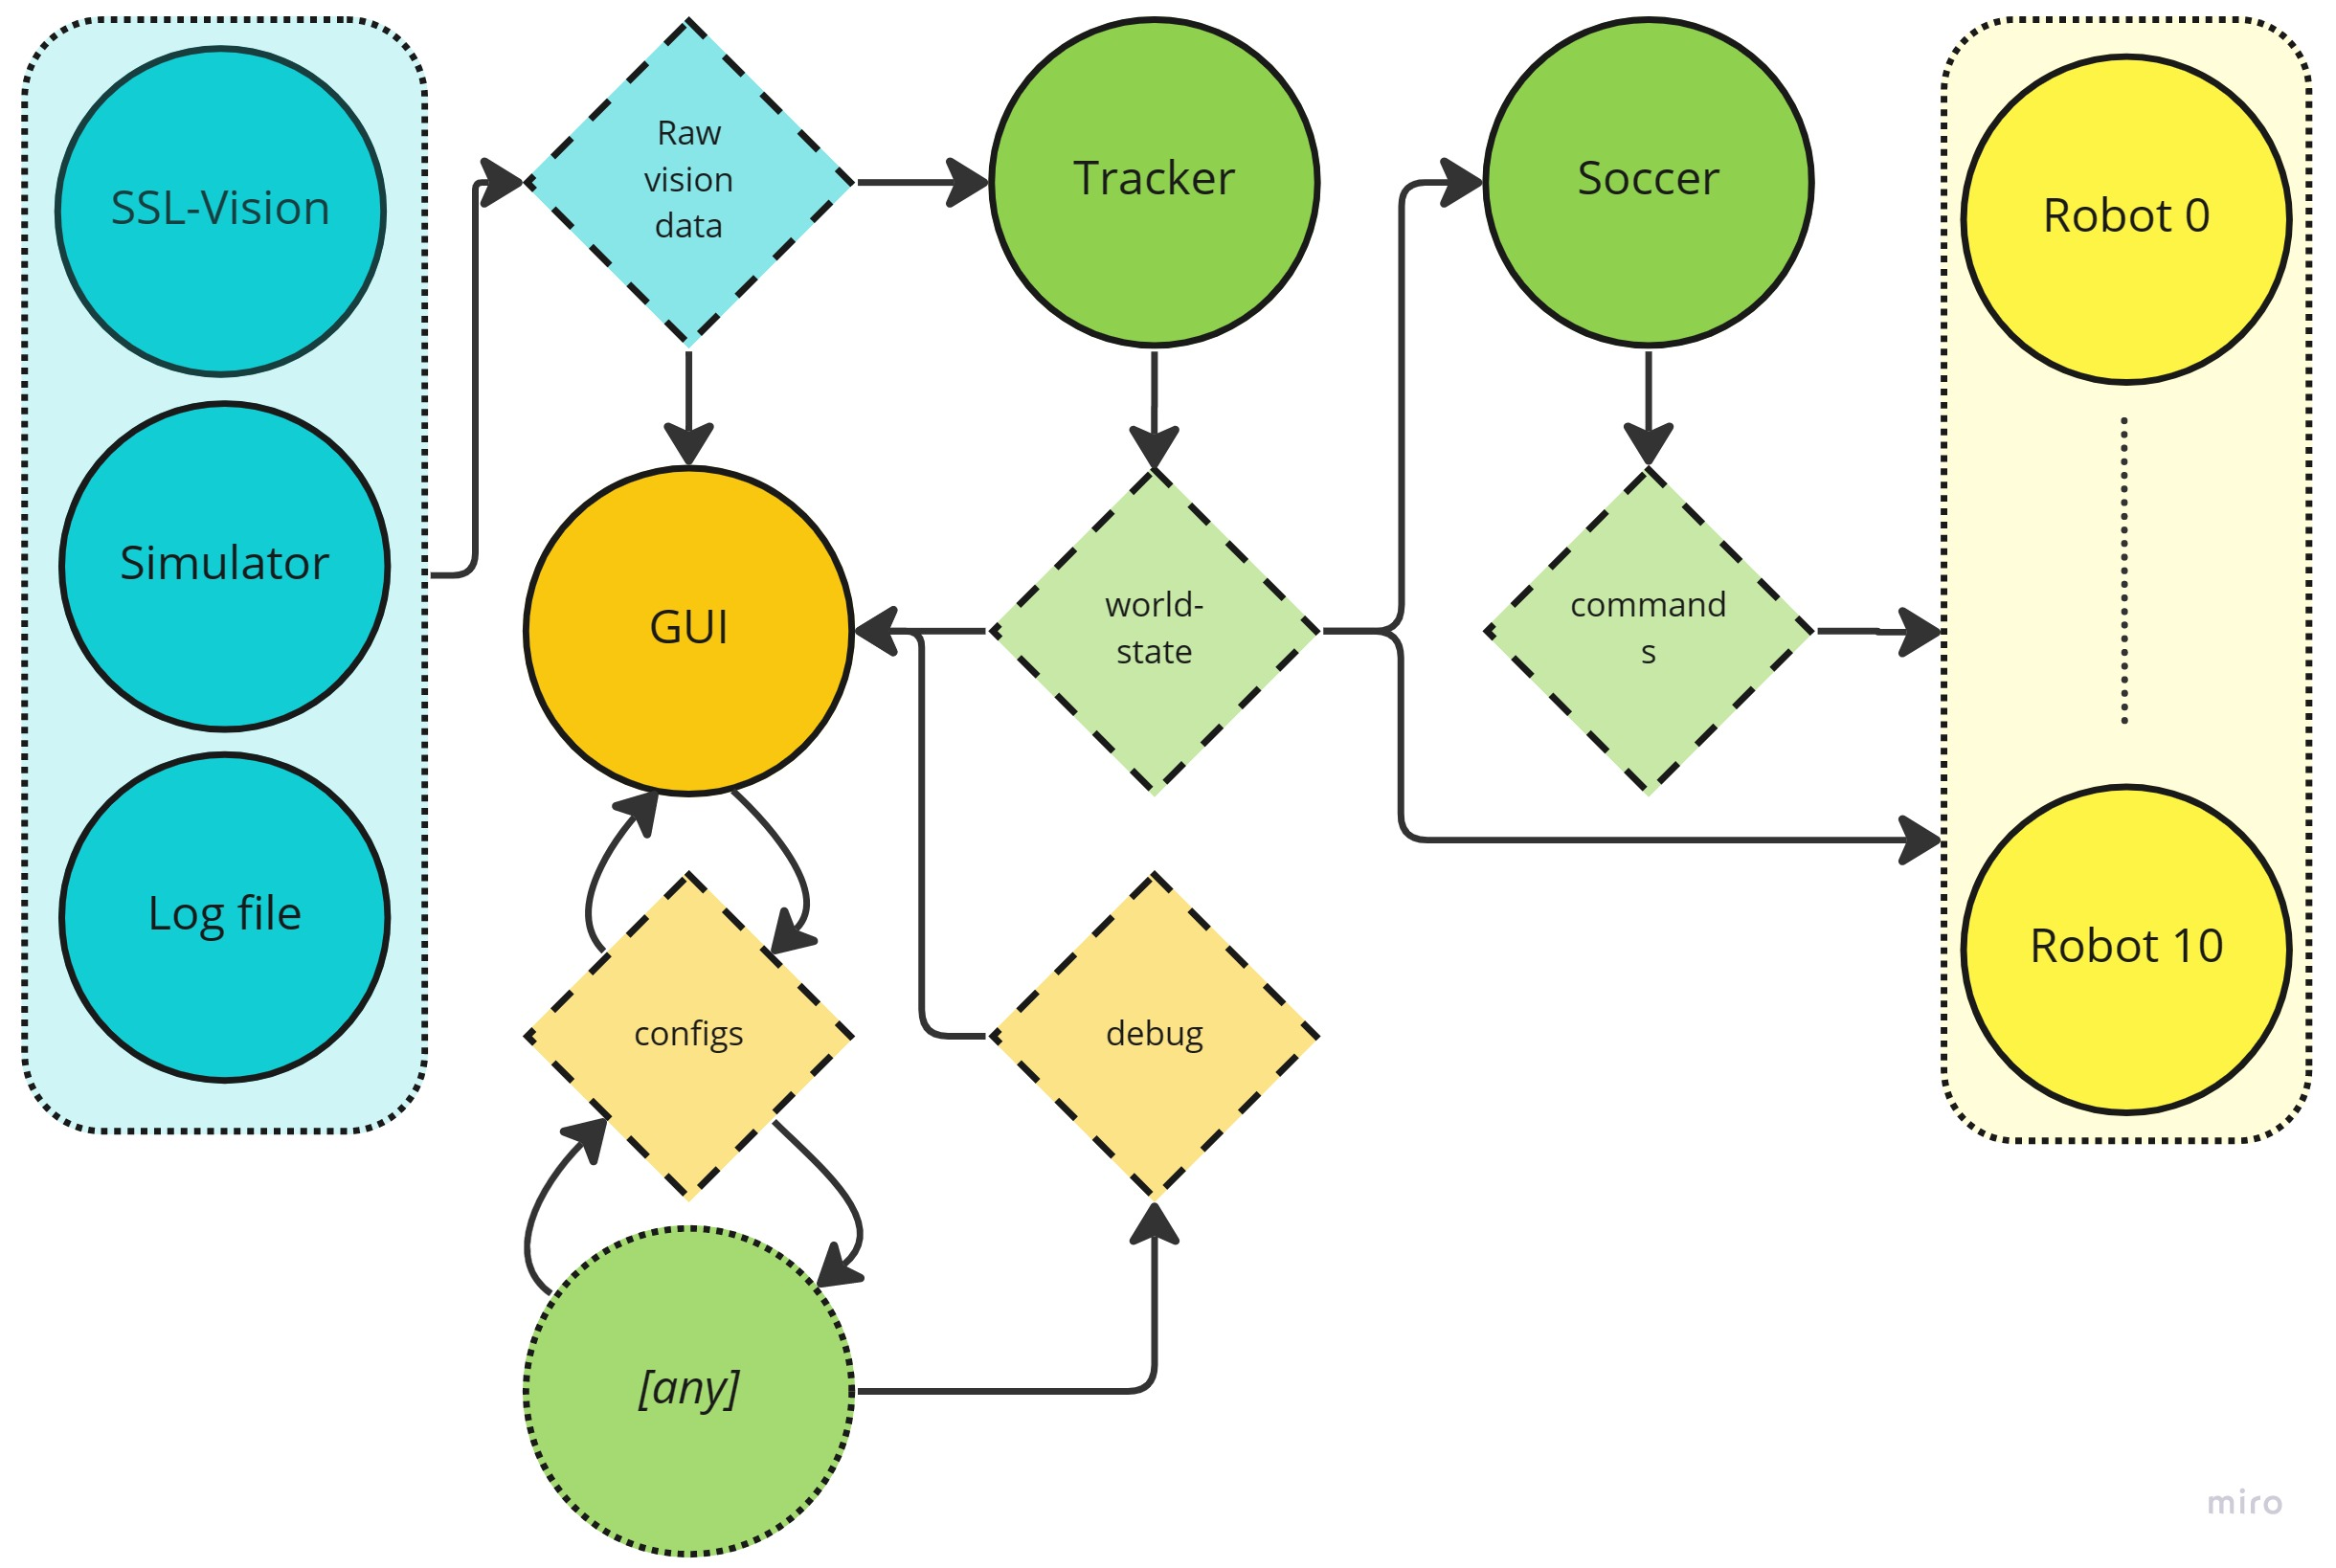
\includegraphics[width=1.0\textwidth]{images/software-architecture.jpg}
	\caption{The new software architecture}
	\label{fig:software-architecture}
\end{figure}

This year the main software also known as the AI software is redesigned in order to be more understandable and extendable. In previous years the software core was the same for each year but with slight changes according to rules and new referee commands. The new members who wanted to implement a new idea in the software needed to spend a great amount of time to understand the methods to use for the robot navigation and data input.

% Written by Omid (We need to merge this with the above soon.

Our team's main focus this year has been on designing a more effective AI system for our robot, with a particular emphasis on improving our debugging process. To achieve this goal, we have redesigned our AI system from the ground up, using C++20 and a modular architecture consisting of three classes: ExternalWorld, WorldState, and Player.

The ExternalWorld class has different subclasses, each of which works in one of the following ways:

\begin{itemize}
\item[$\bullet$] \textbf{RealWorld:} This subclass receives data from a defined SSL-vision and SSL-refbox, and sends robot commands to a defined sender (which forwards the commands to the desired robot).
\item[$\bullet$] \textbf{SimulatedWorld:} This subclass receives data from a defined SSL-vision and SSL-refbox simulator, or any virtual vision or refbox software that adheres to the official protocols of the SSL Communication Protocol, and sends it to a simulator with its own defined protocol.
\item[$\bullet$] \textbf{LogfileWorld:} This subclass receives data from a given logfile of a game. In this mode, the robots act according to the information contained in the logfile without any control. This mode is useful for observing how the player acts in various scenarios. For example, the debugger can show what path each robot would take if it were being controlled by our AI or what strategies to use when the gameplay enters a specific state defined in the logfile.
\end{itemize}

The WorldState class contains all the data describing the state of the game. This includes information about the locations of the robots and ball, as well as the current score and other game details. The ExternalWorld class feeds data to the WorldState module, which uses it to update its internal state.

The Player class is responsible for navigating the robot and generating commands for each robot. This is where the actual AI algorithms are implemented, including path planning, obstacle avoidance, and ball tracking. The Player class uses the data from the WorldState module to make decisions about how to move the robot and interact with other objects in the game.

We have also added both text-based and graphical loggers to our AI system to improve our debugging process. The text-based logger writes output directly to stdout, allowing us to more easily probe exceptions and debug our code. The graphical logger provides us with a visual representation of what the AI software "sees" and how it makes decisions based on the information it has. By utilizing these logging tools, we hope to more effectively debug and refine our AI system.

Throughout the development process, we focused on making our AI software as open and flexible as possible, to allow for easy implementation of new and innovative ideas. We also tested and debugged our software extensively, to ensure that it performs reliably and effectively in different game situations.

%%%%%%%%%%%
\subsection{Finite-State Machine} 
After a few years of experience in the Small Size League as a software designer the key idea that every team is looking to implement is to make the robots to take the correct action at the exact time and condition. If the actions are performed correctly, the robots will accomplish their task which is scoring a goal or preventing the opponent from scoring. Unfortunately, there are many conditions that can happen in a match and each one has its own set of solutions these solutions are the sequence of commands which are given to a set of robots. For the software designer it may be hard to implement the solutions with a group of \textit{IF} conditions and no special structures.

In order to simplify the implementation for multiple software designers in the team, a Finite-State Machine implementation structure has been introduced. This gives a great flexibility and readability of implementation in the code. Each state is connected to other states by a condition or a set of conditions. This makes the implementation easier to probe. By tracking each state transition the faulty part of the code will be simply found.

Each state is basically a function which will be called whenever a complete picture of a field is received from the vision. The input of the function, or state, are the vision data.  
In each state, the set of commands which have to be given to the robots in the field are defined and if there is a condition which a state transition is required the next state will be defined to be called next time.
Table~\ref{tab1} shows a sample group of commands which can be used in every state:

\begin{table}[H]
\caption{Example commands which can be used in every state.}\label{tab1}
\begin{tabular}{|p{7.5cm}|p{6cm}|}
\hline
Function &  Explanation \\
\hline
{\itshape Navigate2Point(robot, destination, maxSpeed)} & Navigate the robot to a destination.\\
{\itshape ERRTNavigate2Point(robot, destination, maxSpeed)} & Navigate the robot while avoiding obstacles.\\
{\itshape Mark(robot, oppRobot)} & Position between the goal and an opponent robot.\\
{\itshape FetchBall(robot, point)} & Navigate the robot to a position on line which the ball is moving on and most close to the \textit{point}.\\
{\itshape OneTouchDirect(robot, point, target)} & Navigate the robot to a position on line which the ball is moving on and most close to the \textit{point}. Kick the ball towards the \textit{target}.\\
{\itshape CircleBall(robot, radius, angle)} & Position robot on a circle around the ball in a specific angle.\\
{\itshape Face(robot, point)} & Face the robot towards a point.\\
{\itshape Chip(robot, power)} & Robot should perform a chip kick whenever the ball was intercepted.\\
{\itshape Direct(robot, power)} & Robot should perform a direct kick whenever the ball was intercepted.\\
{\itshape CircleKickBall(robot, target, power)} & Position robot on a circle around the ball and towards the \textit{target}, then kick the ball.\\
%Title (centered) &  {\Large\bfseries Lecture Notes}\\
%1st-level heading &  {\large\bfseries 1 Introduction}\\
%2nd-level heading & {\bfseries 2.1 Printing Area}\\
%3rd-level heading & {\bfseries Run-in Heading in Bold.} Text follows\\
%4th-level heading & {\itshape Lowest Level Heading.} Text follows\\
\hline
\end{tabular}
\end{table}

As shown in Table~\ref{tab1} the commands are fairly simple to be understood. This simple implementation saves a great amount of time for the programmers to extend or debug the code.

\subsection{Debugging}
Another experience with the previous AI software was the process of debugging the algorithms and, in general, the code itself. To overcome this problem, a logging protocol has been implemented which defines the messages that are sent from the AI software while operating. Using that protocol, whenever a computer is running the AI software while connected to the network, any other computer in the same network can run a logging software and monitor the AI software's parameters including not just the simple inputs from the vision, but also the state, predictions of the algorithms and et al. Fig~\ref{fig_visualizer} shows the graphical visualizer which monitors and records the parameters in the AI software. The visualizer is implement in python while the AI is written in C++ as mentioned before.

\begin{figure}
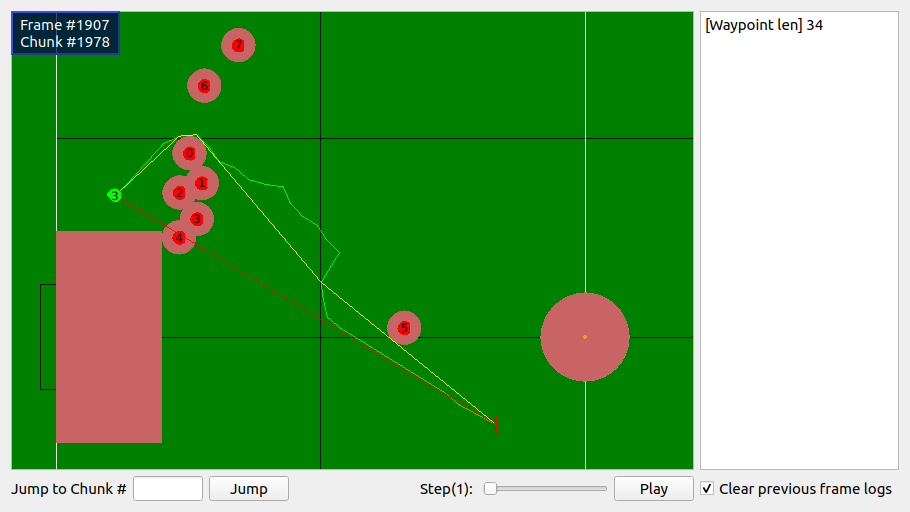
\includegraphics[width=\textwidth]{images/visual1.png}
\caption{A demonstration of the ERRT path plan in the graphical visualizer.} \label{fig_visualizer}
\end{figure}

Fig~\ref{fig1_plotter} shows a simple plotter which  visualizes the changes in the speed and commanded velocity of a single robot. This logging tool is also written in python.

\begin{figure}
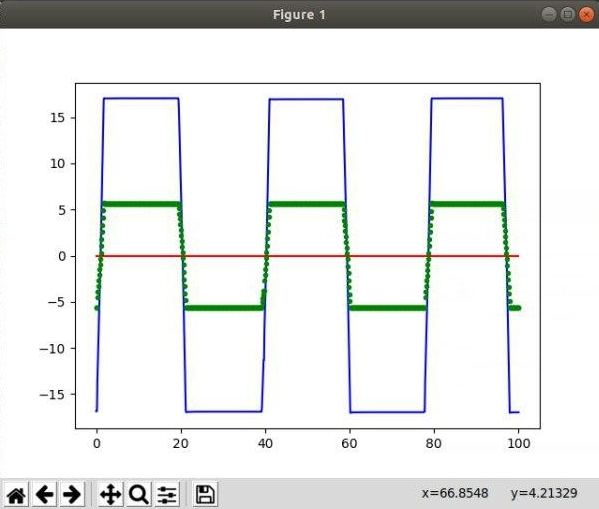
\includegraphics[width=\textwidth]{images/plotter.jpg}
\caption{An example logging program compatible with the new AI software.} \label{fig1_plotter}
\end{figure}

\subsection{Analyzing}
With the tools and designs which were introduced above, it is now possible to demonstrate different features of this project. Below, we will describe the analyzing process in the AI with an example. In the example the goal is to find the best spot in order for a robot to perform a one-touch kick\footnote{A one-touch kick is a robots action where a ball is kicked immediately it touches the front of the robot.}.

There are many parameters to notice while performing a successful one-touch kick (e.g. Initial Ball Velocity, Robots Angle, Velocity of the robot, Target position of the kick). A simple solution to find the optimum values for the parameters is to run tests with different initializations of the parameters. Here, the tests are performed in grSim~\cite{ref_grsim}.

For this example at first, a ball and two robots are stationed at defined locations and a target position is randomly picked in a defined window.

Second, after waiting for a while, one of the robots moves toward the ball and kicks it towards the target position. Meanwhile, the other robot tries to reach to the target position.

Third, After the ball has been moved the second robot is commanded to perform a one touch kick and direct the ball to the center of the goal. This process continues until the ball passes the fields side line or the ball stops moving. If the ball enters the goal, the target position is tagged as a success, in other cases it is tagged as a fail. After this the \textit{round} counter increases by one and the process is repeated from the first state.

At last, After 500 rounds the process is finished and the results are shown in the debugging tools (i.e. the graphical visualizer).

Fig~\ref{fig_ANALYZE_SING_ITR} shows how a single round is performed.

\begin{figure}
\centering
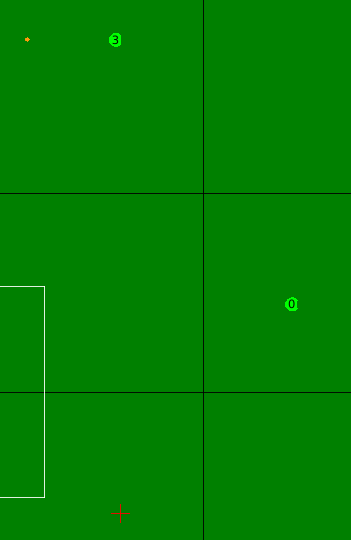
\includegraphics[height=5cm]{images/Analyze_State1.png}
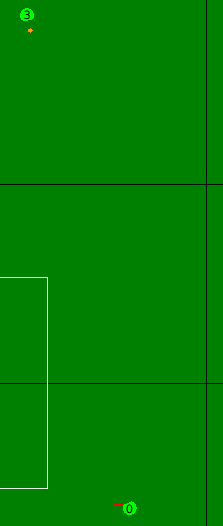
\includegraphics[height=5cm]{images/Analyze_State2.png}
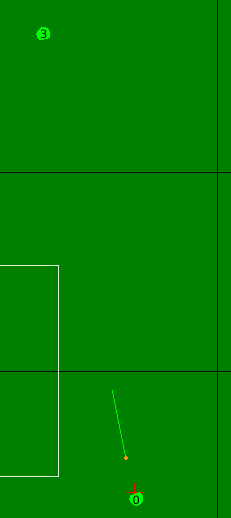
\includegraphics[height=5cm]{images/Analyze_State3.png}
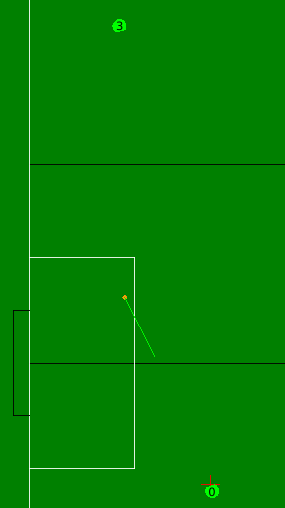
\includegraphics[height=5cm]{images/Analyze_State4.png}\caption{The analysis process shown in the graphical visualizer. Starting from left.} \label{fig_ANALYZE_SING_ITR}
\end{figure}

To define this process the FSM chart shown in Fig~\ref{fig_ANALYZE_FSM} can be implemented in the project\footnote{The chart was drawn in \url{creately.com}}.

\begin{figure}
\centering
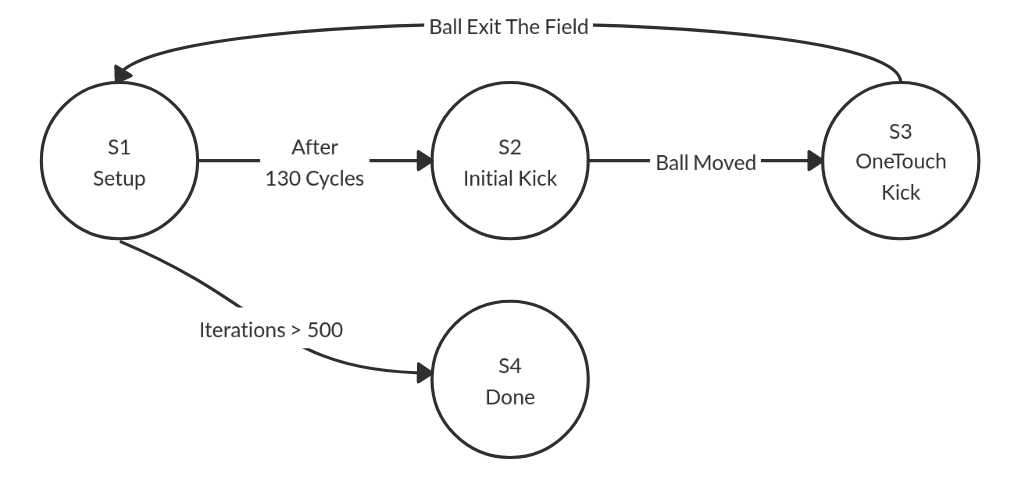
\includegraphics[width=10cm]{images/Analyze_FSM.png}\caption{The FSM chart for the analysis process.} \label{fig_ANALYZE_FSM}
\end{figure}

Now that the FSM is known, each state can be implemented. The pseudocodes of the states are defined in Tables~\ref{table_STATE1_IMP},~\ref{table_STATE2_IMP},~\ref{table_STATE3_IMP} and~\ref{table_STATE4_IMP}. These state functions have access to global variables which are defined in Table~\ref{table_GLOBAL_VARS}.

\begin{table}
\caption{Global variables of the FSM.}
\center
\label{table_GLOBAL_VARS}
\begin{tabular}{|p{10cm}|}
\hline
\textbf{var} 
targetPosition,
initRobotPositions,
initBallPosition,\\
\quad oppGoalPosition:Position;

\textbf{var}
round, cnt:int;

\textbf{var}
successPositions,failPositions:Position[];

\textbf{var}
nextFunc2Run:function;\\

\hline
\end{tabular}
\end{table}

In Table~\ref{table_GLOBAL_VARS}, the \textit{targetPosition} is the location where the robot will perform its one-touch kick. This variable is initialized in every round. 

The \textit{initRobotPositions} and \textit{initBallPosition} are the initial locations of the robots and the ball in every round. These variables are defined before the start of the test. \textit{oppGoalPosition} is the position of the center of the opponents goal line. This variable is defined before the start of the test.

\textit{successPositions} and \textit{failPositions} are two vectors which store the positions according to their tags, \textbf{fail} or \textbf{success}.

\textit{nextFunc2Run} is the function which will run in the next cycle (i.e. The next time a new vision dataset is received). This variable is defined as a C++ pointer to function in our executable code.


\begin{table}[H]
\caption{Implementation of the \textit{Setup} state.}
\center
\label{table_STATE1_IMP}
\begin{tabular}{|p{10cm}|}
\hline

\textbf{function}
$ S1\_setup$()\\
\quad placeRobots(initRobotPositions);\\
\quad placeBall(initBallPosition);\\
\quad targetPosition = pickRandomPosition();\\
\quad logData();\\
\quad \textbf{if} round >= 500 \textbf{then}\\
\quad\quad nextFunc2Run := S4\_done;\\
\quad\quad cnt := 0;\\
\quad \textbf{else if} cnt >= 130 \textbf{then}\\
\quad\quad nextFunc2Run := S2\_initKick;\\
\quad\quad cnt := 0;\\
\quad \textbf{else}\\
\quad\quad cnt := cnt + 1;\\

\hline
\end{tabular}
\end{table}

In \textit{S1\_setup}(), the robots and the ball have to get placed in the specified positions. This can be done by replacing the balls by hand or by robots and at last navigating the robots towards the specified positions.
If the test is being performed in a simulator (e.g. grSim) it is possible to immediately place the robot by a command. Since the current test is performed in grSim, the robots will be placed using the placement commands implemented in grSim. These commands are shown as \textit{initRobotPositions}() and \textit{initBallPosition}() in the pseudocode. In every cycle (i.e. every time the function is called) A variable called \textit{cnt} is incremented by one. It is checked in an if statement to check whether it is time to transit to the next state or to stay in the current state. Another if statement checks if the round number has reached to 500, if so, the FSM will transit to the \textit{done} state which brings the process to an end.

\begin{table}[H]
\caption{Implementation of the \textit{Initial Kick} state.}
\center
\label{table_STATE2_IMP}
\begin{tabular}{|p{10cm}|}
\hline

\textbf{function}
$ S2\_initKick$()\\
\quad circleKickBall(Robot3, targetPosition, 100);\\
\quad ERRTNavigate2Point(Robot0, targetPosition);\\
\quad logData();\\
\quad \textbf{if} cnt >= 5 \textbf{then}\\
\quad\quad nextFunc2Run := S3\_oneTouchKick;\\
\quad\quad cnt := 0;\\
\quad \textbf{else if} ballIsMoving() \textbf{then}\\
\quad\quad cnt := cnt + 1;\\

\hline
\end{tabular}
\end{table}

In \textit{S2\_initKick}(), Robot \#3 tries to aim the \textit{targetPosition} and kick the ball towards it. Meanwhile, Robot \#0 will try to reach the \textit{targetPosition}. After a few moments when the ball is moving, the FSM will transit to the next state.


\begin{table}[H]
\caption{Implementation of the \textit{OneTouchKick} state.}
\center
\label{table_STATE3_IMP}
\begin{tabular}{|p{10cm}|}
\hline

\textbf{function}
$ S3\_oneTouchKick$()\\
\quad halt(Robot3);\\
\quad oneTouchDirect(Robot0, targetPosition, oppGoalPosition);\\
\quad logData();\\
\quad \textbf{if} ballIsOut() \textbf{then}\\
\quad\quad \textbf{if} ballInGoal() \textbf{then}\\
\quad\quad\quad successPositions.add(targetPosition);\\
\quad\quad \textbf{else} \\ 
\quad\quad\quad failPositions.add(targetPosition);\\
\quad\quad nextFunc2Run := S1\_setup;\\
\quad\quad round := round + 1;\\
\quad \textbf{else if} ballIsNotMoving() \textbf{then}\\
\quad\quad failPositions.add(targetPosition);\\
\quad\quad nextFunc2Run := S1\_setup;\\
\quad\quad round := round + 1;\\

\hline
\end{tabular}
\end{table}

In \textit{S3\_oneTouchKick}(), Robot \#3 gets into a halt mode and Robot \#0 will wait for the ball to reach it. Once the ball gets fetched by the robot. it will get kicked towards the \textit{oppGoalPosition}. The state transition will not happen until the ball exits the field or stops moving. When one of the transition conditions happen it will be judged whether the test was a success or a fail according to the position of the ball in relation with the goal.

\begin{table}[H]
\caption{Implementation of the \textit{Done} state.}
\center
\label{table_STATE4_IMP}
\begin{tabular}{|p{10cm}|}
\hline

\textbf{function}
$ S4\_done$()\\
\quad halt(Robot3);\\
\quad halt(Robot0);\\
\quad logData();\\
\quad logData(successPositions, GREEN);\\
\quad logData(failPositions, RED);\\

\hline
\end{tabular}
\end{table}

In \textit{S4\_done}(), the robots are halted and the results are sent to the visualizer as red and green points.

After running the code with 500 rounds in 1 hour and 20 minutes, the results were shown on the visualizer with 142 successful and 358 failed attempts. Fig~\ref{fig_ANALYZE_OUTPUT} shows the visualizer at the end of the test. It is now clearly seen which areas have a high possibility in scoring a goal by a one-touch kick under the tested conditions.

\begin{figure}[H]
\centering
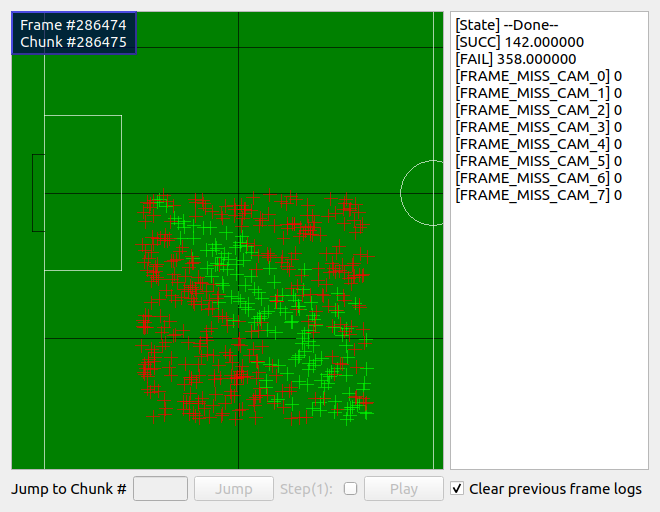
\includegraphics[width=10cm]{images/Analyze_output.png}\caption{The final results of the analysis.} \label{fig_ANALYZE_OUTPUT}
\end{figure}

Finally, it is worth to notice that the test has been performed in a simulation to give a better result in a short amount of time. It is clear that this test has to be made on robots in the real world. In that case, the number of rounds will obviously need to decrease to a few tens. The focus of this section was to show how an analysis procedure is taken in the Immortals AI project.

%\section{3D printed robot}
%As mentioned in the previous years team description papers~\cite{ref_ETDP2019,ref_ETDP2018}, A new type of robot was introduced to the league by this team in order to reduce the time and energy for manufacturing the robots.
%
%The design of the 3d printed robots where published and are available for teams and individuals to use~\cite{ref_opensource}. The designs are being updated to increase robustness. However, the robustness of a 3d printed robot is incomparable with a usual SSL robot which is assembled with metal parts. Teams may choose to build this type of robot in order to run tests which require a high number of robots.

%\begin{figure}
%\centering
%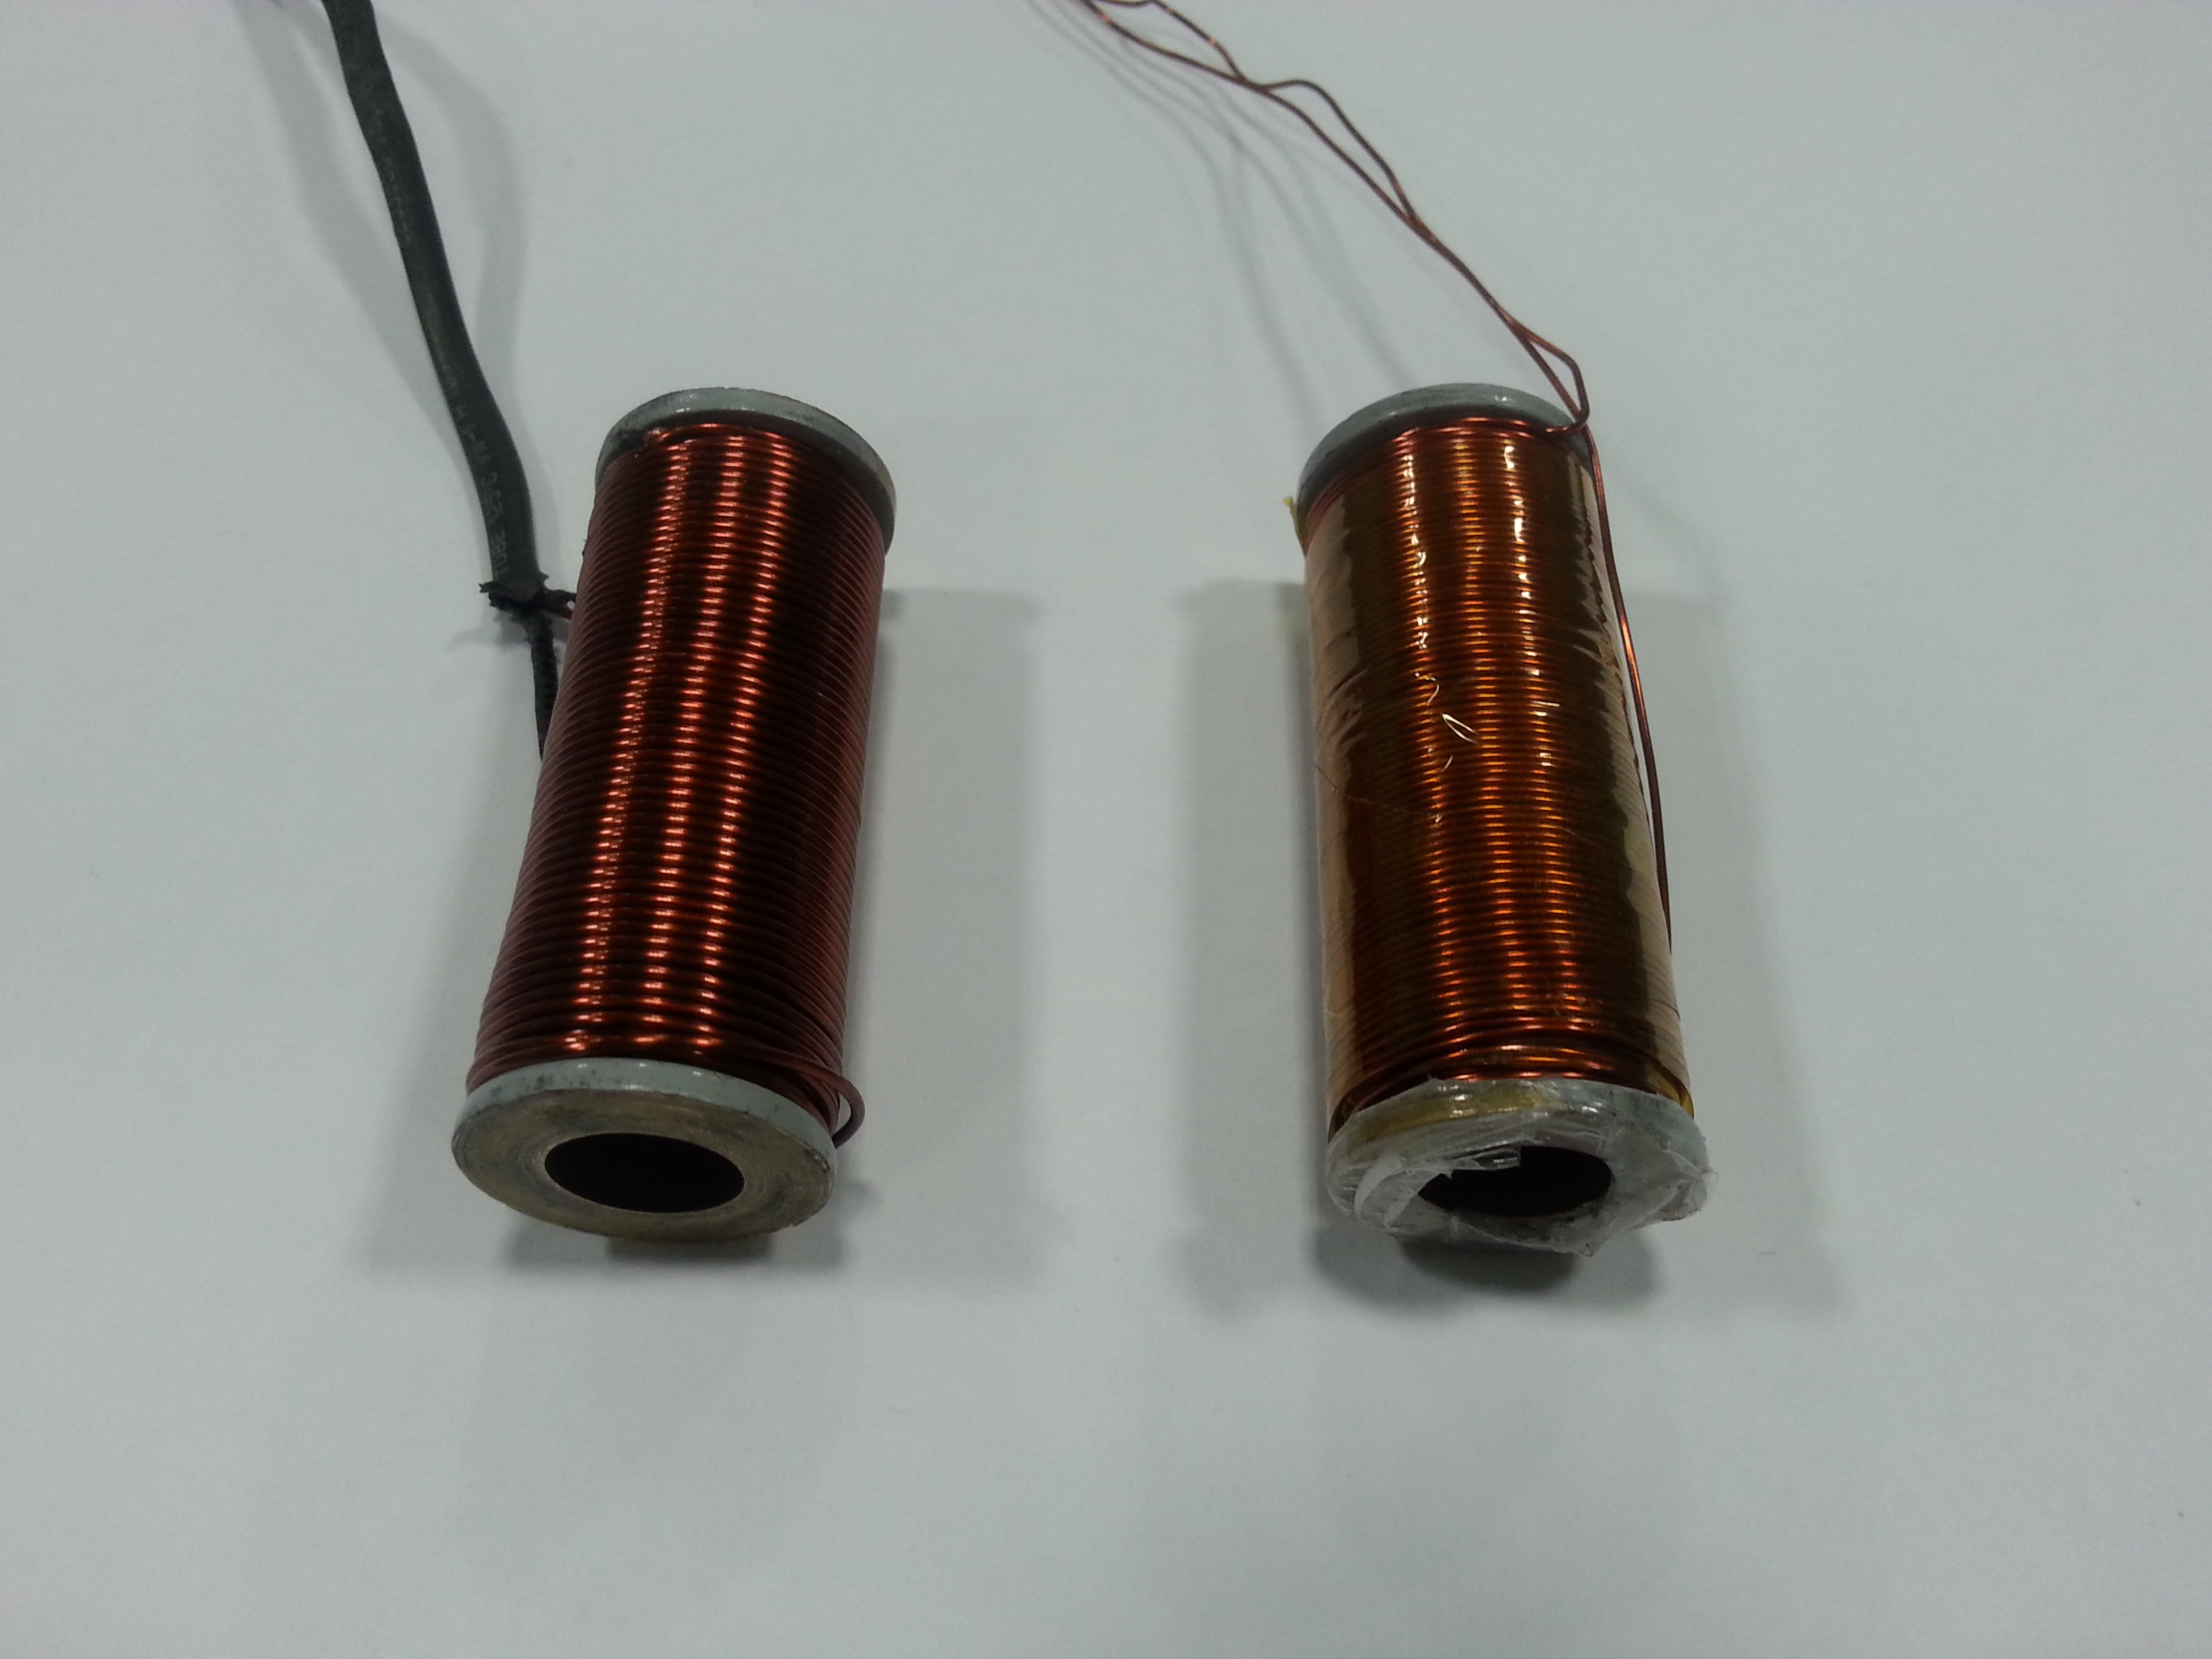
\includegraphics[width=10cm]{images/solenoid.jpg}
%\caption{The old solenoid(Left) and the new solenoid(Right).} \label{fig_solenoid}
%\end{figure}


%\begin{figure}
%\centering
%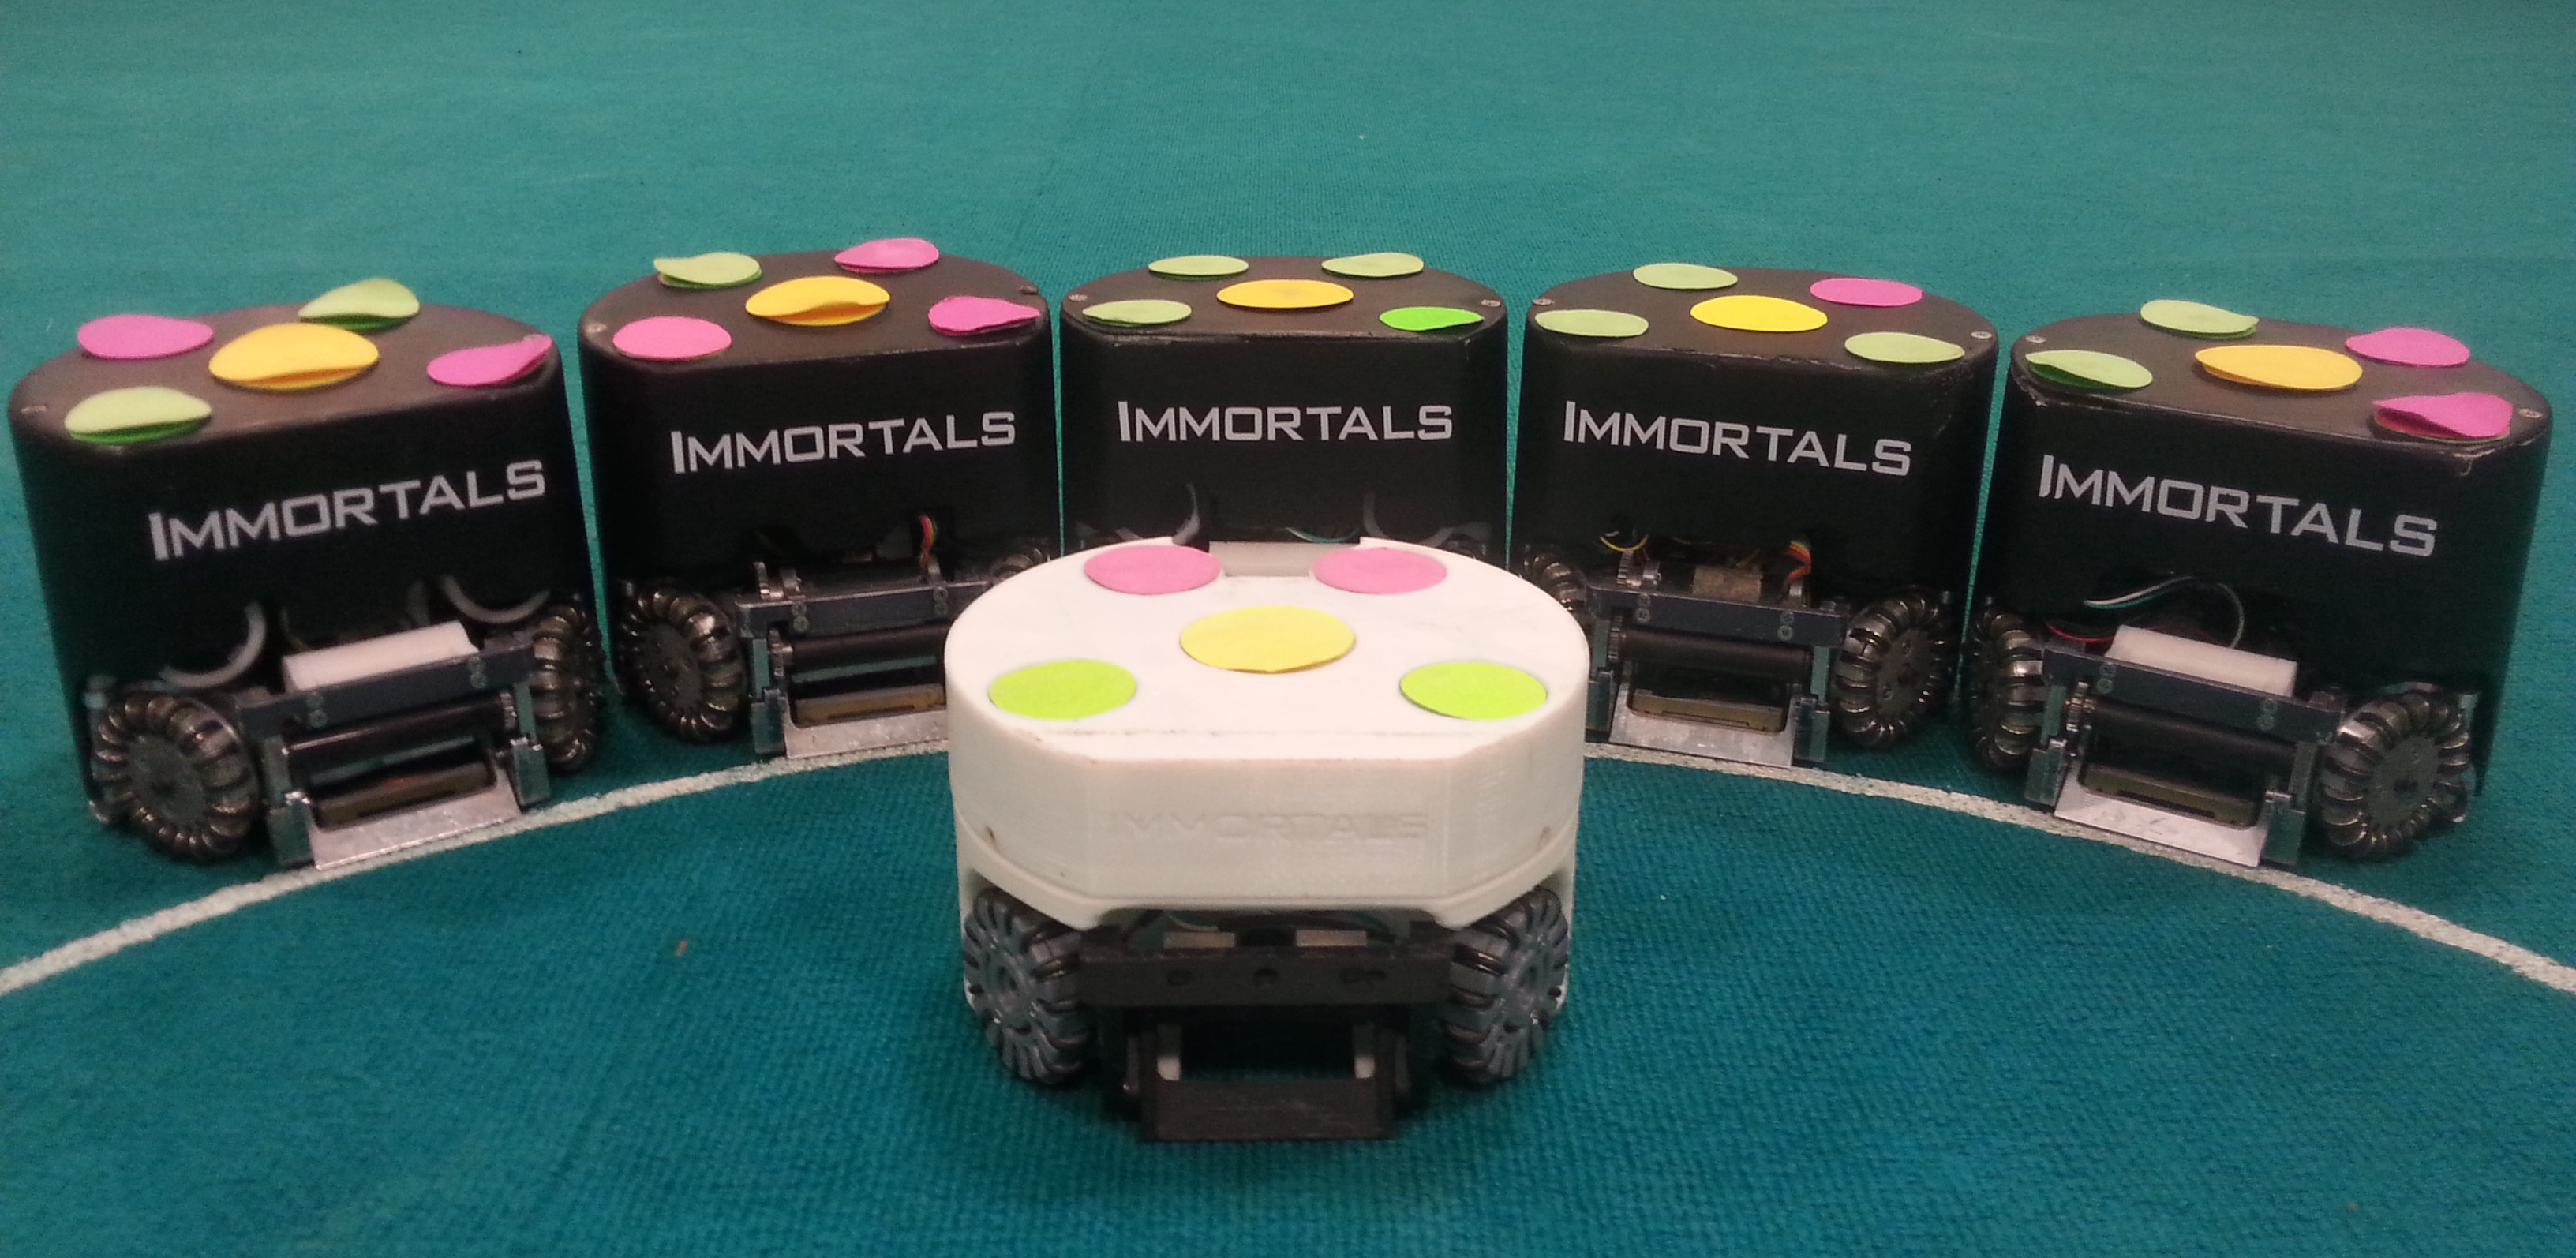
\includegraphics[width=10cm]{images/5plus1.jpg}
%\caption{Five old robots and a single 3D printed robot at the front.} \label{fig_5plus1}
%\end{figure}



\newpage
\begin{thebibliography}{8}
\bibitem{ref_website}
Immortals Robotics Website, \url{http://www.immortals-robotics.com}.

\bibitem{ref_ETDP2020}
Immortals 2020 Extended Team Description Paper, \url{https://ssl.robocup.org/wp-content/uploads/2020/03/2020\_ETDP\_Immortals.pdf}.

\bibitem{ref_ETDP2019}
Immortals 2019 Team Description Paper, \url{https://ssl.robocup.org/wp-content/uploads/2019/03/2019\_ETDP\_Immortals.pdf}.

\bibitem{ref_ETDP2018}
Immortals 2018 Team Description Paper, \url{https://ssl.robocup.org/wp-content/uploads/2019/01/2018\_TDP\_Immortals.pdf}.

\bibitem{ref_opensource}
Immortals Open Source Project. \url{https://github.com/Ma-Ghasemieh/Immortals\_ssl\_opensource\_mech}.

\bibitem{ref_opensource}
Immortals Open Source Publish in RoboCup 2016. \url{https://github.com/lordhippo/immortalsSSL}.

\bibitem{ref_grsim}
Monajjemi, Valiallah (Mani), Ali Koochakzadeh, and Saeed Shiry Ghidary. "grSim – RoboCup Small Size Robot Soccer Simulator." In Robot Soccer World Cup, pp. 450-460. Springer Berlin Heidelberg, 2011.

% 3rd-party libraries
\bibitem{ref_3rd-party_asio}
Asio, cross-platform C++ library for network and low-level I/O programming \url{https://think-async.com/Asio/}

\bibitem{ref_3rd-party_quill}
Quill, asynchronous Low Latency C++ Logging Library \url{https://github.com/odygrd/quill}

\bibitem{ref_3rd-party_tomlplusplus}
toml++, header-only TOML config file parser and serializer for C++17. \url{https://github.com/marzer/tomlplusplus}

\bibitem{ref_3rd-party_eigen}
Eigen, C++ template library for linear algebra \url{https://eigen.tuxfamily.org/}

\bibitem{ref_3rd-party_homog2d}
homog2d, C++ 2D geometry library \url{https://github.com/skramm/homog2d}

\end{thebibliography}
\end{document}
